\documentclass[10pt,a4paper]{article}
\usepackage[utf8]{inputenc}
\usepackage[italian]{babel}
\usepackage{amsmath}
\usepackage{amsfonts}
\usepackage{amssymb}
\usepackage{graphicx}
\usepackage[left=2cm,right=2cm,top=2cm,bottom=2cm]{geometry}
\newcommand{\rem}[1]{[\emph{#1}]}

\author{Gruppo xx \\ Andrea Luzio, Gianfranco Cordella, Valerio Lomanto}
\title{Esercitazione N.1: Misure di tensione, corrente, tempi, frequenza.}
\begin{document}

\maketitle

\section{Scopo e strumentazione}

L'esercitazione ha lo scopo di impratichirsi con la strumentazione e le tecniche di misura. 
Abbiamo utilizzato sia il multimetro digitale sia il tester analogico. 

\section{Misure di tensione e corrente}
\paragraph{2.b Partitore}
Abbiamo montato il circuito in Fig. 1\footnote{della scheda "Esercitazione N.1"} con i valori di resistenza misurati con il multimetro digitale: $R_1 = 810\pm 7 \Omega$ e $R_2 = 1.116\pm 0.01 k\Omega$. L'errore \`e stato stimato usando le indicazioni del manuale del multimetro ($0.8\%$ + 1 cifra). 
Dall'analisi del circuito ci aspettiamo che $V_\mathrm{OUT}/V_\mathrm{IN} = \frac{1}{1+R_1/R_2}= 1.70 \pm 0.01  $.


Variando $V_\mathrm{IN}$ abbiamo ottenuto i dati riportati in tabella.

\begin{table}[h]
\centering
\begin{tabular}{|c|c|c|c|}
\hline 
VIN[V]& $\sigma$ VIN[mV] &VOUT[V]	 & $\sigma$ VOUT[mV] \\
\hline 
10.40 & 60 & 6.12 & 40 \\
9.00 & 55 & 5.29 & 30 \\
7.3 & 46 & 4.3 & 30 \\
5.16 & 35 & 3.03 & 25 \\
3.73 & 28 & 2.19 & 21 \\
1.94 & 10 & 1.14 & 6 \\
0.575 & 4 & 0.338 & 3 \\
\hline 
\end{tabular} 
\caption{Partitore di tensione con resistenze da circa 1k. Tutte le tensioni in V.\label{t:par1}}
\end{table}
\begin{figure}
\centering
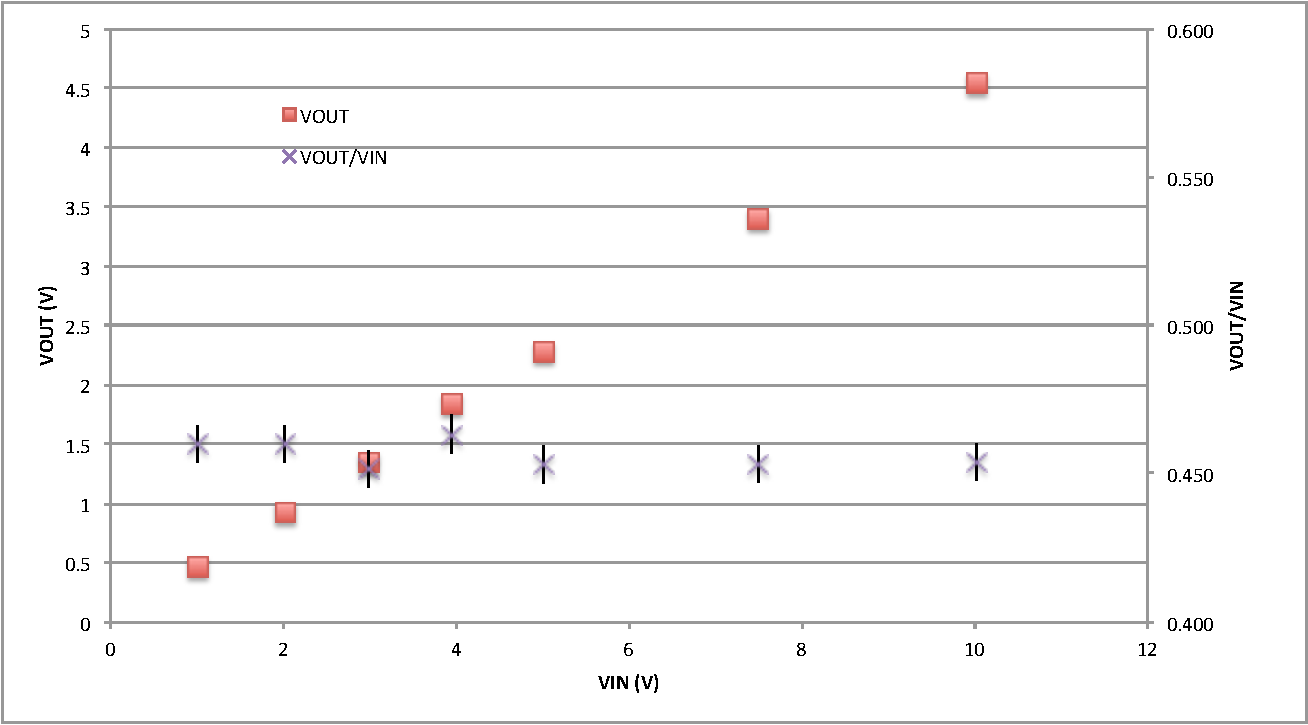
\includegraphics[scale=0.4]{part1.pdf}
\caption{Partitore di tensione.\label{f:par1}}
\end{figure}
Come ci si aspettava la relazione tra tensione di ingresso ed uscita \`e lineare. Il rapporto $V_{OUT}/V_{IN}=1.700 \pm 0.006$ \`e da confrontare con il valore aspettato indicato sopra.

\paragraph{2.c Partitore con resistenze più grandi}
Montando di nuovo il partitore con le resistenze $R_1 = 1.518\pm 0.01 M\Omega$ e $R_2 = 1.03\pm 0.01 M\Omega$, usando il voltmetro analogico per misurare $V_{OUT}$($20 kohm/volt$) si osservano i nuovi dati in tabella 2
\begin{table}[h]
\centering
\begin{tabular}{|c|c|c|c|}
\hline 
VIN[V]& $\sigma$ VIN[mV] & VOUT[V]	 & $\sigma$ VOUT[mV] \\
\hline 
10.02 & 60 & 0.24 & 2 \\
8.90 & 55 & 0.20 & 2 \\
7.90 & 50 & 0.18 & 1 \\
6.80 & 44 & 0.16 & 1 \\
6.06 & 40 & 0.14 & 1 \\
4.52 & 30 & 0.1 & 0.6 \\
3.52 & 30 & 0.08 & 0.5 \\
\hline 
\end{tabular} 
\caption{Partitore di tensione. Tutte le tensioni in V.\label{t:par2}}
\end{table}
\begin{figure}
\centering
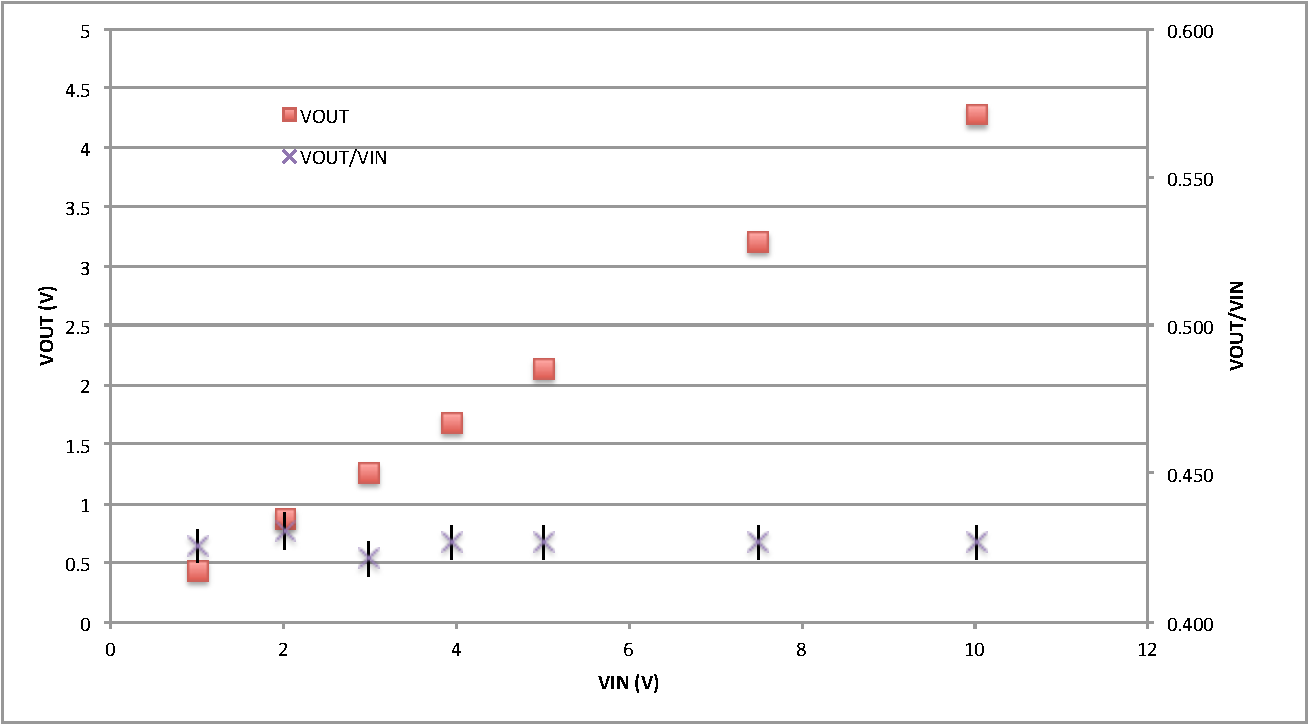
\includegraphics[scale=0.4]{part2.pdf}
\caption{Partitore di tensione con resistenze da circa 1M.\label{f:par2}}
\end{figure}

Si osserva come valore del rapporto misurato con le resistenze da $1 M\Omega$, $0.0229 \pm 1e-04$ si discosti da quanto atteso   $V_\mathrm{OUT}/V_\mathrm{IN} = \frac{1}{1+R_1/R_2}= 0.40 $\footnote{\'E stato omesso l'errore poich\'e il calcolo \'e stato fatto senza considerare la resistenza di ingresso del voltmetro, li risultato \'e tuttavia chiaramente incompatibile con l'ipotesi che il voltmetro sia uno strumento ideale}. La ragione della discrepanza \`e da ricercarsi nella impedenza di ingresso del tester.


\paragraph{2.d Resistenza di ingresso del tester}

 Usando il modello mostrato nella scheda si ottiene
\[ \frac{R_1}{R_T} =  \frac{V_{IN}}{V_{OUT}} - (1 +  \frac{R_1}{R_2} )
\]
Il valore misurato \'e dunque $R_T=38.3 \pm 0.6 kohm$, vicino ai valori di riferimento del tester analogico( $40 kohm$ con il fondoscala $2 V$, dato fornito dal manuale senza incertezza).

\subsection{Partitore di corrente: 2.e}

Si monta il circuito indicato con i valori di resistenza misurati con il multimetro digitale: 
$R_3= 98.3\pm 1 k\Omega$, $R_1 = 560\pm 5 \Omega$, $R_2 = 220\pm 3 \Omega$.
Si \'e variata la tensione fornita dal generatore nel range $20-10 V$ per ottenere pi\'u misure e poter procedere con un fit.
Il valore di tensione $V_{in}$ \'e stato misurato con il multimetro digitale, mentre la corrente con l'analogico, fornendo esso misure pi\'u precise per basse correnti in continua.\\
 

\begin{center}
\begin{tabular}{|c|c|c|c|c|c|}
\hline 
$V_{in} (V)$ & $\sigma V_{in} (V)$& I1 ($\mu A$)& $\sigma$(I1) ($\mu A$) & I2	($\mu A$) & $\sigma$(I2) ($\mu A$)  \\
\hline 
19.2 & 0.1 & 26.0 & 0.3 & 10.0 & 0.1 \\
17.2 & 0.1 & 23.5 & 0.2 & 9.0 & 0.1 \\
14.9 & 0.1 & 20.5 & 0.2 & 8.0 & 0.1 \\
12.65 & 0.07 & 17.0 & 0.2 & 7.00 & 0.07 \\
10.87 & 0.06 & 15.00 & 0.15 & 6.00 & 0.06 \\
\hline 
\end{tabular} 
\end{center}

Ci si accorge subito che $I_1=I_{tot,1}\frac{R_2}{R_{int}+R_1+R_2}$ (dove $R_{int}$\footnote{dove $I_{tot, 1}$ \'e la corrente che passa da $R_3$ quando l'amperometro \'e nel ramo di $R_1$, similmente $I_{tot, 2}$ } \'e la resistenza interna dell'amperometro, c.a. $2 kohm$ con il fondoscala usato). Anche $I_2=I_{tot,2}\frac{R_1}{R_{int}+R_1+R_2}$. \'E lecito approssimare $I_{tot, 1}=I_{tot, 2}=I_{tot}$ poich\'e la resistenza $R_3$ domina sul parallelo in entrambi i casi.
Dalle equazioni scritte sopra si nota che $\frac{I_1}{I_2}=\frac{R_2}{R_1}$ ma non \'e vero che $I_1+I_2=I_{tot}$. Infatti sperimentalmente(facendo un fit lineare ad un parametro, si veda figura 1 e 2, di $I_1=K I_2$:
$\frac{I_1}{I_2}=1.99 \pm 0.05$
compatibile con il valore atteso di $\frac{R_2}{R_1}=2.00 \pm 0.02$.
\begin{figure}
\centering
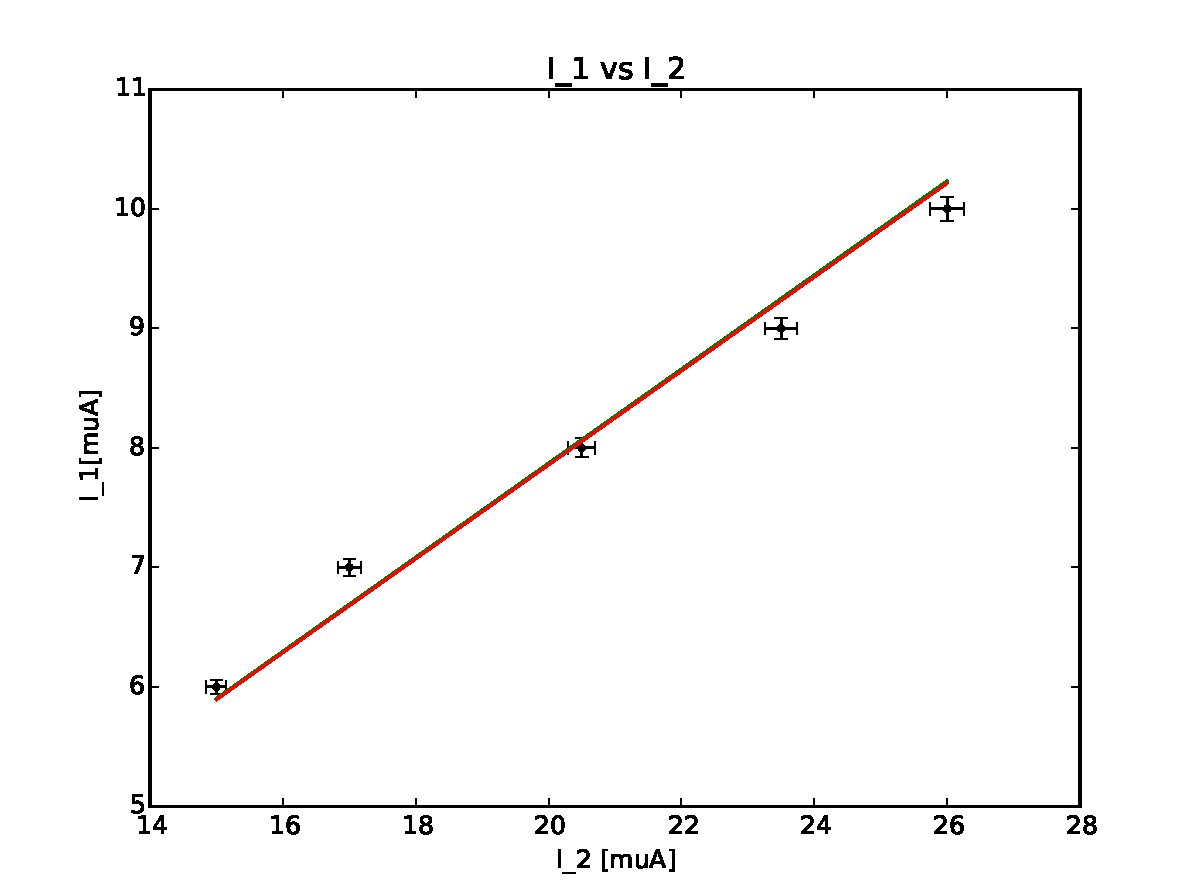
\includegraphics{./immagini/fig2e.pdf}
\caption{Fit e dati di $I_1 vs I_2$}
\end{figure}
\begin{figure}
\centering
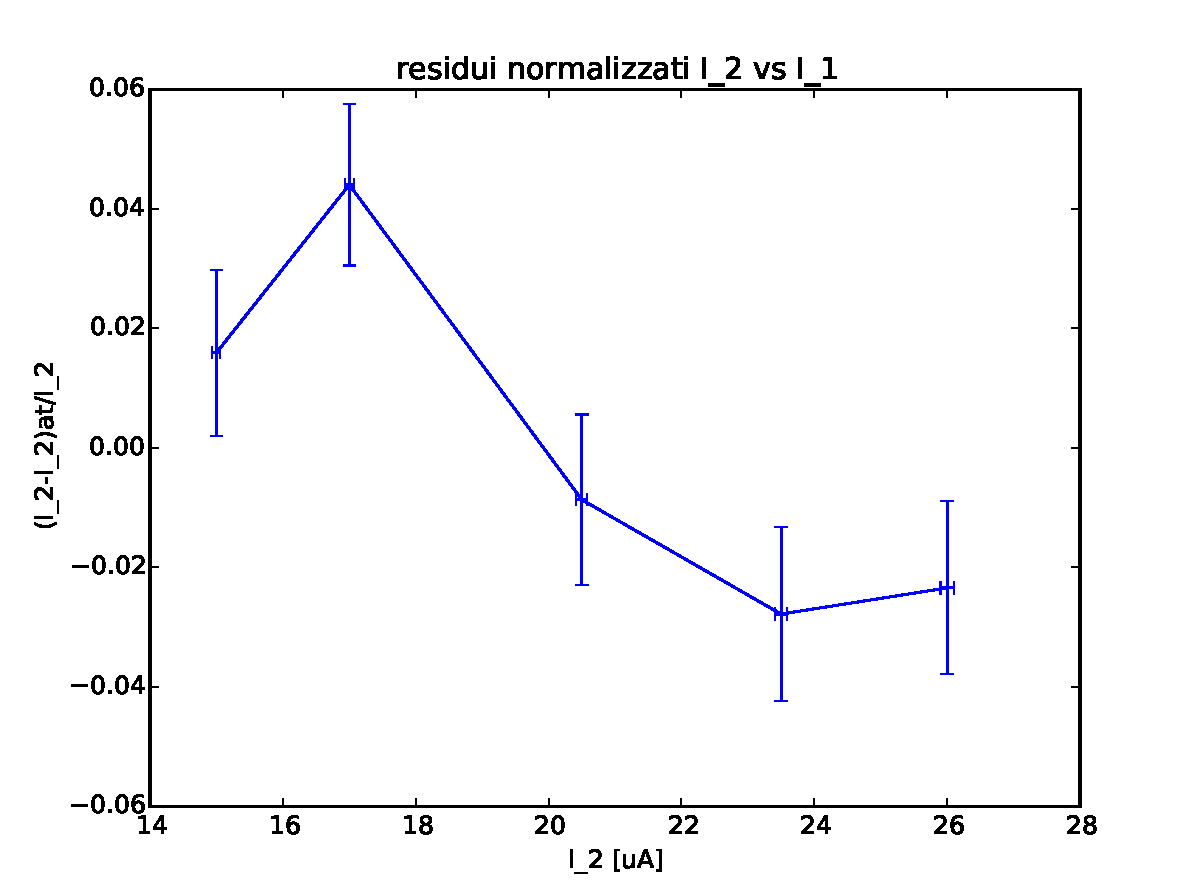
\includegraphics{./immagini/fig2eres.pdf}
\caption{Residui di $I_1 vs I_2$}
\end{figure}
Chiaramente $I_1+I_2\neq I_{tot}$ ad esempio, per la prima misura, $\frac{I_1+I_2}{I_{tot}}=0.18$
Si pu\'o calcolare, sfruttando questa discrepanza la resistenza interna dell'amperometro. Sempre nell'approssimazione che $I_{tot}$ non cambi spostando l'amperometro (questo \'e vero con un incertezza maggiore del 0.5 \%) la resistenza interna dell'amperometro \'e $R_A = (R1+R2)\left(\frac{I_{TOT}}{I1+I2} - 1 \right)$. Dunque $R_A=3.4 kohm$ al $1.2 \%$.



\section{Uso dell'oscilloscopio}

\paragraph{Misure di tensione}
Usando i seguenti resistori per fare un partitore di tensione $ 
R_2=9.91\pm 0.08 kohm
R_1=9.90\pm 0.08 kohm$
si ottengono le seguenti misure:
\begin{table}[h]
\centering
\begin{tabular}{|c|c|c|c|}
\hline 
VIN[V]& $\sigma$ VIN[mV] &VOUT[V]	 & $\sigma$ VOUT[mV] \\
\hline 
11.6 & 0.7 & 5.92 & 0.3 \\
9.8 & 0.6 & 4.8 & 0.3 \\
8.1 & 0.4 & 4.0 & 0.2 \\
5.4 & 0.3 & 2.7 & 0.14 \\
4.2 & 0.2 & 2.1 & 0.1 \\
2.64 & 0.14 & 1.33 & 0.07 \\
1.76 & 0.10 & 0.88 & 0.05 \\
\hline 
\end{tabular} 
\caption{Partitore di tensione usato con l'oscilloscopio.\label{t:par1}}
\end{table}
Il rapporto di partizione misurato \'e $1.99\pm 0.04 $ contro un valore atteso di $2.00 \pm 0.02$.


\paragraph{Impedenza di ingresso dell'oscilloscopio}
L'impedenza di ingresso dell'oscilloscopio \'e stata misurata con un partitore di tensione con $R_1=0.985\pm 0.01 Mohm R_2=0.560\pm 0.005 Mohm$. Il CH2 dell'oscilloscopio (quello del quale abbiamo misurato l'impedenza di ingresso) era ai capi di $R_1$. Con CH1 si misurava invece la tensione di ingresso al partitore.
La resistenza risultante \'e $1.0 \pm 0.1 Mohm$.  

\section{Misure di frequenza e tempo}
Sono stati misurate le seguenti frequenze:
\begin{table}[h]
\centering
\begin{tabular}{|c|c|c|c|}
\hline 
$f_{oscilloscopio}[kHz] $& $f[kHz]$ &$\sigma f [kHz]$ \\
\hline 
1.559 & 1.53 & 0.01 \\
15.09 & 15.3 & 0.1 \\
150.4 & 148 & 1 \\
1506.0 & 1490 & 10 \\

\hline 
\end{tabular} 
\caption{Frequenze misurate con il frequenzimetro e con i cursori. Non \'e noto l'errore del frequenzimetro.\label{t:par1}}
\end{table}

\section{Trigger dell'oscilloscopio}
Generando un onda quadra con frequenza $1 MHz$ si sono ottenuti i seguenti tempi di salita e discesa:


\begin{table}[h]
\centering
\begin{tabular}{|c|c|c|}
\hline 
tipo misura& manuale[ns] & automatico[ns] \\
\hline 
salita & $68 \pm 1$ & $66 \pm 2$ \\
discesa & $62 \pm 1$ & $62 \pm 2$\\

\hline 
\end{tabular} 
\caption{La misura automatica \'e presa con l'opportuna funzione dell'oscilloscopio, la manuale con i cursori. \label{t:par1}}
\end{table}
\section{Conclusioni e commenti finali}
Di questa esperienza non abbiamo capito molto, sfortunatamente non abbiamo fatto saltare alcun fusibile. 

\end{document}